\documentclass[]{beamer}
\usepackage[T1]{fontenc}
\usepackage[utf8]{inputenc}
\usepackage{lmodern}
\usepackage[italian]{babel}

\title{L'entropia}
\author{\texorpdfstring{Mattia Cozzi\newline\href{mailto:cozzimattia@gmail.com}{\texttt{cozzimattia@gmail.com}}}{Mattia Cozzi}}
\date{a.s.~2023/2024}

%\documentclass[handout]{beamer}     %usare questa classe per generare l'handout
%\usepackage{pgfpages}   %per mostrare più quadri nella stessa pagina
%\pgfpagesuselayout{4 on 1}[a4paper,border shrink=5mm,landscape]
\usetheme{Singapore}
%\useoutertheme[left]{sidebar} %elementi intorno alle diapositive
\setbeamercovered{dynamic} %modifica l'aspetto del testo grigetto delle diapositive future. Argomenti: invisible/transparent/dynamic
\usecolortheme{orchid}
%COLORE PRINCIPALE
% \definecolor{marroncino}{RGB}{156, 26, 0} % UBC Blue (primary)
% \setbeamercolor{structure}{fg=marroncino} % itemize, enumerate, etc
%
\theoremstyle{plain}
\newtheorem{teorema}{Teorema}

\usepackage{tikz}


\usepackage{pgf,pgfplots,graphicx}
\usetikzlibrary{angles,quotes,arrows,shapes,decorations.markings}
\pgfplotsset{compat=1.15}
\usepgfplotslibrary{units,fillbetween} % to add units easily to axis
\tikzset{fleche/.style args={#1:#2}{postaction=decorate,decoration={name=markings,mark=at position #1 with {\arrow[#2,scale=2]{>}}},},}



\begin{document}

\begin{frame}
  \titlepage
\end{frame}





\begin{frame}
\frametitle{Contenuti}
\tableofcontents
\end{frame}


\section{Clausius (2)}

\begin{frame}
\frametitle{``Qualità'' del calore}
Consideriamo due macchine di Carnot A e B.{\pause} Le due macchine hanno la \alert<2>{stessa sorgente fredda} a temperatura $ T_1 = 300 \, K $ e prelevano $ Q_B = Q_A = 100 \, J $ di calore dalla sorgente calda.\pause
\\~\\
Le due macchine differiscono per la \alert<3>{temperatura della sorgente calda}: $ T_A = 400 \, K $, mentre $ T_B = 600 \, K $.
\\~\\\pause
Ricordiamo che per la macchina di Carnot vale:
\begin{center}
\colorbox{blue!30}{$ \eta = 1 - \dfrac{T_1}{T_2} $}
\end{center}
\end{frame}

\begin{frame}
\frametitle{``Qualità'' del calore}
\begin{columns}
\begin{column}{0.45\textwidth}
\begin{center}
$ \eta_A = 1 - \frac{300 \, K}{400 \, K} = \dfrac{1}{4} $
\end{center}
\begin{figure}
\begin{tikzpicture}[scale=0.4]
\node [above,purple] at (0,1.5) {A};
\draw [purple, ultra thick] (0,0) circle [radius=1.5];
\draw (-4,1) -- (-4,-1);
\draw (-4,1) -- (-5.5,1);
\draw (-4,-1) -- (-5.5,-1);
\node [left,red] at (-4,0) {{\scriptsize $ 400 \, K $}};

\draw (4,1) -- (4,-1);
\draw (4,1) -- (5.5,1);
\draw (4,-1) -- (5.5,-1);
\node [right,blue] at (4,0) {{\scriptsize $ 300 \, K $}};

\draw [->,thick,red] (-4,0) -- (-1.5,0);
\node [below,red] at (-2.75,0) {{\scriptsize $ 100 \, J $}};

\draw [->,thick,blue] (1.5,0) -- (4,0);
\node [below,blue] at (2.75,0) {{\scriptsize $ 75 \, J $}};

\draw [->,thick] (0,-1.5) -- (0,-3);
\node [right] at (0,-2.25) {{\scriptsize $ 25 \, J $}};
\end{tikzpicture}
\end{figure}

\end{column}
\begin{column}{0.45\textwidth}
\begin{center}
$ \eta_B = 1 - \frac{300 \, K}{600 \, K} = \dfrac{1}{2} $
\end{center}
\begin{figure}
\begin{tikzpicture}[scale=0.4]
\node [above,purple] at (0,1.5) {B};
\draw [purple, ultra thick] (0,0) circle [radius=1.5];
\draw (-4,1) -- (-4,-1);
\draw (-4,1) -- (-5.5,1);
\draw (-4,-1) -- (-5.5,-1);
\node [left,red] at (-4,0) {{\scriptsize $ 600 \, K $}};

\draw (4,1) -- (4,-1);
\draw (4,1) -- (5.5,1);
\draw (4,-1) -- (5.5,-1);
\node [right,blue] at (4,0) {{\scriptsize $ 300 \, K $}};

\draw [->,thick,red] (-4,0) -- (-1.5,0);
\node [below,red] at (-2.75,0) {{\scriptsize $ 100 \, J $}};

\draw [->,thick,blue] (1.5,0) -- (4,0);
\node [below,blue] at (2.75,0) {{\scriptsize $ 50 \, J $}};

\draw [->,thick] (0,-1.5) -- (0,-3);
\node [right] at (0,-2.25) {{\scriptsize $ 50 \, J $}};
\end{tikzpicture}
\end{figure}

\end{column}
\end{columns}
~\\~\\
\visible<2>{Possiamo intuitivamente affermare che i $ 100 \, J $ della macchina B sono più ``preziosi'', nel senso che permettono di produrre più lavoro. Ciò è causato dalla alta temperatura della sorgente calda della macchina B.}

\end{frame}

\begin{frame}
\frametitle{Calore e temperatura}
Per comprendere il comportamento del calore alle diverse temperature Rudolf Clausius nel 1864 introdusse il concetto di \alert<1>{entropia}.{\pause} Partiamo dal teorema di Carnot:
\begin{center}
$ \eta \leq \eta_{rev} $\\~\pause\\
$ 1- \frac{|Q_1|}{Q_2} \leq 1 - \frac{T_1}{T_2} $\\~\pause\\
$ \frac{Q_2}{T_2} \leq \frac{|Q_1|}{T_1} $\\~\pause\\ 
$ \frac{Q_2}{T_2} \leq - \frac{Q_1}{T_1} $\\~\pause\\
$ \frac{Q_2}{T_2} + \frac{Q_1}{T_1} \leq 0 $
\end{center}
\end{frame}


\begin{frame}
  \frametitle{La disuguaglianza di Clausius}
  Generalizzando il risultato precedente, possiamo scrivere:
  \begin{center}
  \colorbox{blue!30}{$ \sum\limits_{i=1}^n \left( \frac{\Delta Q_i}{T_i} \right) \leq 0 $}
  \end{center}
  dove l'uguale vale solo se la macchina termica è reversibile.

\end{frame}
\section{Entropia}

\begin{frame}
  \frametitle{Una nuova grandezza}
  \begin{center}
  $ \sum\limits_{i=1}^n \left( \frac{\Delta Q_i}{T_i} \right) \leq 0 $
  \end{center}
  Il termine che vediamo variare tra parentesi nella disuguaglianza di Clausius è detto \alert<1>{entropia} (simbolo $ S $) e si misura in $ \frac{J}{K} $.{\pause}
  \begin{alertblock}{Attenzione}
  Essendo l'entropia introdotta mediante la sua variazione, il livello zero dell'entropia può essere scelto arbitrariamente (vedremo più avanti quale è la convenzione).    
  \end{alertblock}
\end{frame}

\begin{frame}
  \frametitle{L'entropia}
    \begin{block}{Definizione}
    L'entropia $ S(A) $ di un sistema $ A $ è data dalla variazione di entropia tra lo stato $ R $ di riferimento (a entropia zero) e lo stato $ A $.
    \begin{center}
    $ S(A) = S(A) - 0 = S(A) - S(R) = \left( \sum\limits_{i=1}^n \frac{\Delta Q_i}{T_i}  \right)_{R \rightarrow A}^{rev}  $
    \end{center}
  \end{block}
\end{frame}

\begin{frame}
  \frametitle{Cosa è l'entropia}
  L'entropia è:
  \begin{itemize}
    \item una \alert<1>{grandezza estensiva}, cioè una grandezza che varia con il variare delle \emph{dimensioni} del sistema (lo sono anche la massa e il volume, ma non la densità o la temperatura);\pause
    \item una \alert<2>{funzione di stato};\pause
    \item utilizzabile per \alert<3>{interpretare statisticamente} il secondo principio della termodinamica.
  \end{itemize}
\end{frame}



\begin{frame}
  \frametitle{Cosa non è l'entropia}
  L'entropia non è:
  \begin{itemize}
    \item una \alert<1>{grandezza misteriosa}: è oggetto della fisica, e pertanto è misurabile come ogni altro ente fisico;\pause
    \item né il \alert<2>{disordine} né l'assenza di esso, anche se è utilizzata per distinguere forme ordinate di energia e forme non ordinate;\pause
    \item utilizzabile nel medesimo senso della fisica in \alert<3>{altri contesti} (come le scienze sociali), a meno di non reinterpretarla in senso non fisico.
  \end{itemize}
\end{frame}


\begin{frame}
\frametitle{Entropia di un sistema isolato (1)}
  Immaginiamo di avere un sistema isolato in cui una \alert{trasformazione irreversibile} porta il sistema da uno stato $ A $ ad uno stato $ B $ e successivamente una \alert{trasformazione reversibile} riporta il sistema allo stato $ A $.{\pause} Vale:
\begin{center}
$ \left( \sum\limits \frac{\Delta Q_i}{T_i}  \right)_{A \rightarrow B}^{irr} + \left( \sum\limits \frac{\Delta Q_i}{T_i}  \right)_{B \rightarrow A}^{rev} \leq 0  $
\end{center}
La definizione di entropia ci dice che $ \left( \sum\limits \frac{\Delta Q_i}{T_i}  \right)_{B \rightarrow A}^{rev} = S(A) - S(B) $ e pertanto:
\begin{center}
$ \left( \sum\limits \frac{\Delta Q_i}{T_i}  \right)_{A \rightarrow B}^{irr} + S(A) - S(B) \leq 0 $
\end{center}
\end{frame}



\begin{frame}
\frametitle{Entropia di un sistema isolato (2)}
\begin{center}
$ \left( \sum\limits \frac{\Delta Q_i}{T_i}  \right)_{A \rightarrow B}^{irr} + S(A) - S(B) \leq 0 $
\end{center}
Le diverse parti del sistema possono scambiare calore tra loro, ma essendo il sistema isolato ogni termine della sommatoria sarà nullo, e pertanto:\pause
\begin{center}
  \colorbox{blue!30}{$ S(A) \leq S(B) $}
\end{center}\pause
Detto altrimenti, l'entropia di un sistema isolato è sempre \emph{non decrescente}.{\pause} In particolare:
\begin{itemize}
  \item se le trasformazioni sono reali, l'entropia è crescente;
  \item se le trasformazioni sono ideali, l'entropia è costante.
\end{itemize}
\end{frame}





\begin{frame}
\frametitle{Entropia dell'universo}
Se consideriamo l'intero Universo, esso è certamente un sistema isolato in cui avvengono trasformazioni irreversibili, e pertanto l'entropia dell'universo è sempre in aumento.\pause
\\~\\
Osservazione, utile per l'interpretazione statistica dell'entropia di un sistema: il tempo scorre nel verso a cui corrisponde un aumento di entropia.
\end{frame}






\section{Spontaneità}

\begin{frame}
  \frametitle{Prevedere il futuro}
  Immaginiamo di avere un sistema isolato nello stato $ A $, e che $ A $ non sia uno stato di equilibrio. Lasciamo il sistema libero di evolversi e assistiamo a dei cambiamenti.{\pause\\~\\} Come possiamo prevedere lo stato finale del sistema? Ci sono moltissimi stati possibili del sistema in accordo con la conservazione dell'energia.\pause\\~\\
  Per esempio, il principio di conservazione dell'energia ammette come possibile che un corpo, se sollevato, rilasci la sua energia potenziale sotto forma di calore. Perché questo di fatto non accade?
\end{frame}


\begin{frame}
  \frametitle{Variazione di entropia}
  Sappiamo che ad ognuno di questi stati possibili raggiungibili dallo stato $ A $ corrisponderà una certa variazione di entropia.\\~\pause\\
  Gli esperimenti e la teoria che vedremo tra poco mostrano che lo stato raggiunto spontaneamente dal sistema è quello a cui corrisponde il \alert<2>{massimo aumento dell'entropia}.  
\end{frame}


\begin{frame}
  \frametitle{Una nuova formulazione per il secondo principio}
  Sulla base di quanto detto, possiamo enunciare il secondo principio della termodinamica in un quarto modo, anch'esso logicamente equivalente agli altri tre:\pause
  \begin{block}{Enunciato dell'entropia}
    L'evoluzione spontanea di un sistema isolato giunge a uno stato di equilibrio a cui corrisponde il massimo aumento dell’entropia (compatibile con il rispetto del primo principio della termodinamica).
  \end{block}
\end{frame}





\begin{frame}
\frametitle{Entropia di un sistema non isolato}
Recuperiamo un esempio già visto, il frigorifero: se consideriamo come sistema l'interno del frigorifero, durante il processo di raffreddamento avremo $ \Delta Q < 0  $, e pertanto $ \Delta S < 0 $.\\~\pause\\
Sappiamo tuttavia che ciò non avviene in modo \emph{spontaneo}, è necessario un apporto energetico esterno.\\~\pause\\Le serpentine calde del frigorifero, se operassero trasformazioni ideali, renderebbero la variazione di entropia del sistema-Universo nulla. Poiché operano trasformazioni reali, la variazione di entropia nel sistema-Universo risulti ancora una volta positiva.
\end{frame}


\begin{frame}
  \frametitle{Osservazioni}
  Possiamo notare una profonda \emph{asimmetria nella natura}:
  \begin{itemize}
    \item i trasferimenti di calore avvengono spontaneamente dai corpi caldi a quelli freddi e non viceversa (Clausius);
    \item è possibile la completa conversione del lavoro in calore, ma non il contrario (Kelvin).
  \end{itemize}\pause
Mentre un sistema evolve nel tempo, l'entropia aumenta e le differenze di temperatura diminuiscono, e pertanto diminuisce il lavoro massimo estraibile dal calore (esempio iniziale). Possiamo in effetti pensare allora che l'entropia permetta di dare una sorta di misura della ``qualità'' dell'energia.\\\pause~\\
Prima di scoprire il perché di questo fenomeno, riflettiamo sui concetti di \emph{disordine} e di \emph{tempo}.
\end{frame}



\section{Disordine}


\begin{frame}
  \frametitle{Energia ordinata ed energia disordinata}
\begin{columns}
\begin{column}{0.5\textwidth}
\visible<1->{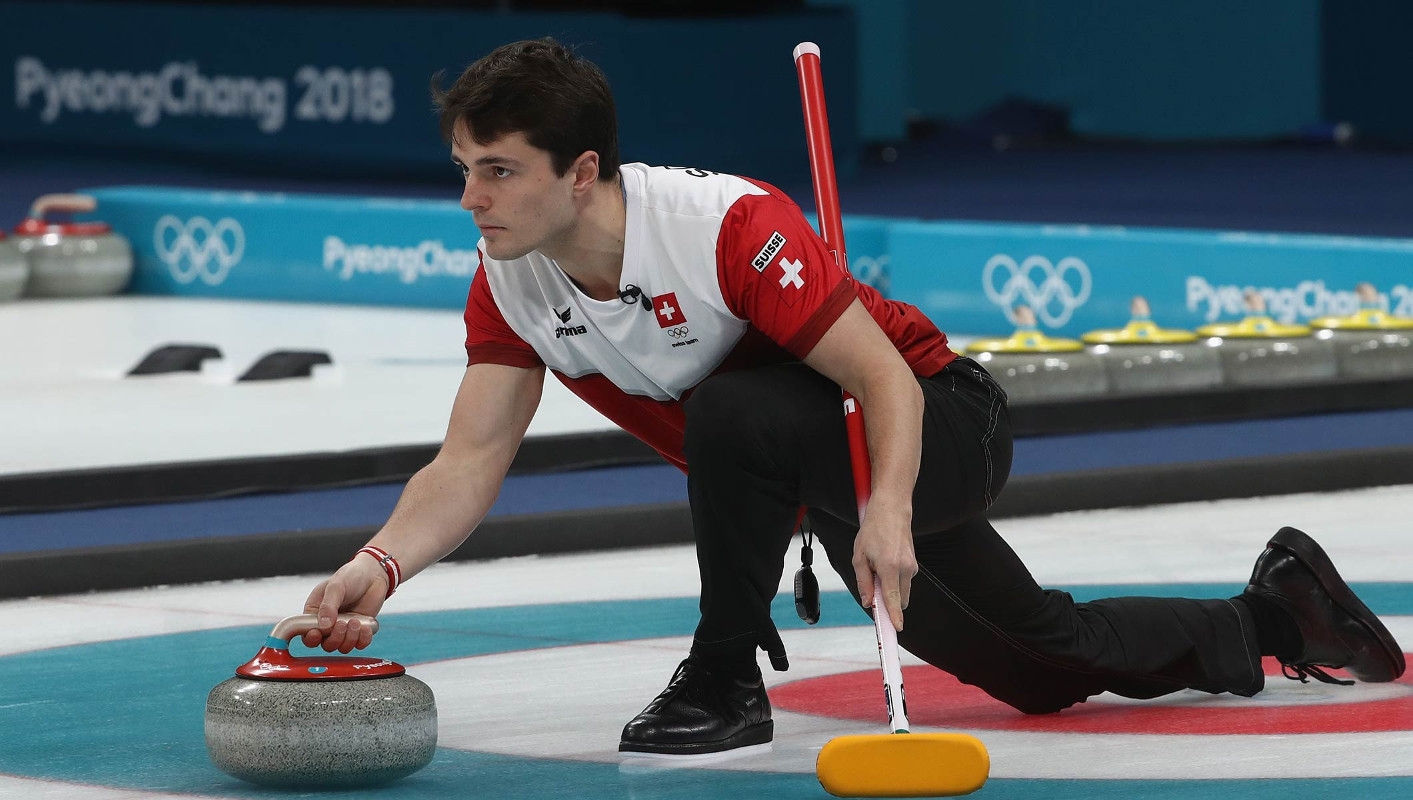
\includegraphics[width=\columnwidth]{img/curling.jpg}}
{\footnotesize Il giocatore di \emph{curling} dona alla pietra \emph{energia cinetica}, una forma di \alert{energia ordinata}; infatti:
\begin{itemize}
  \item vi contribuiscono tutte le molecole della pietra;
  \item le molecole si muovono tutte con la stessa velocità;
  \item le molecole si muovono tutte nella stessa direzione.
\end{itemize}}
\end{column}
\begin{column}{0.5\textwidth}
\visible<2->{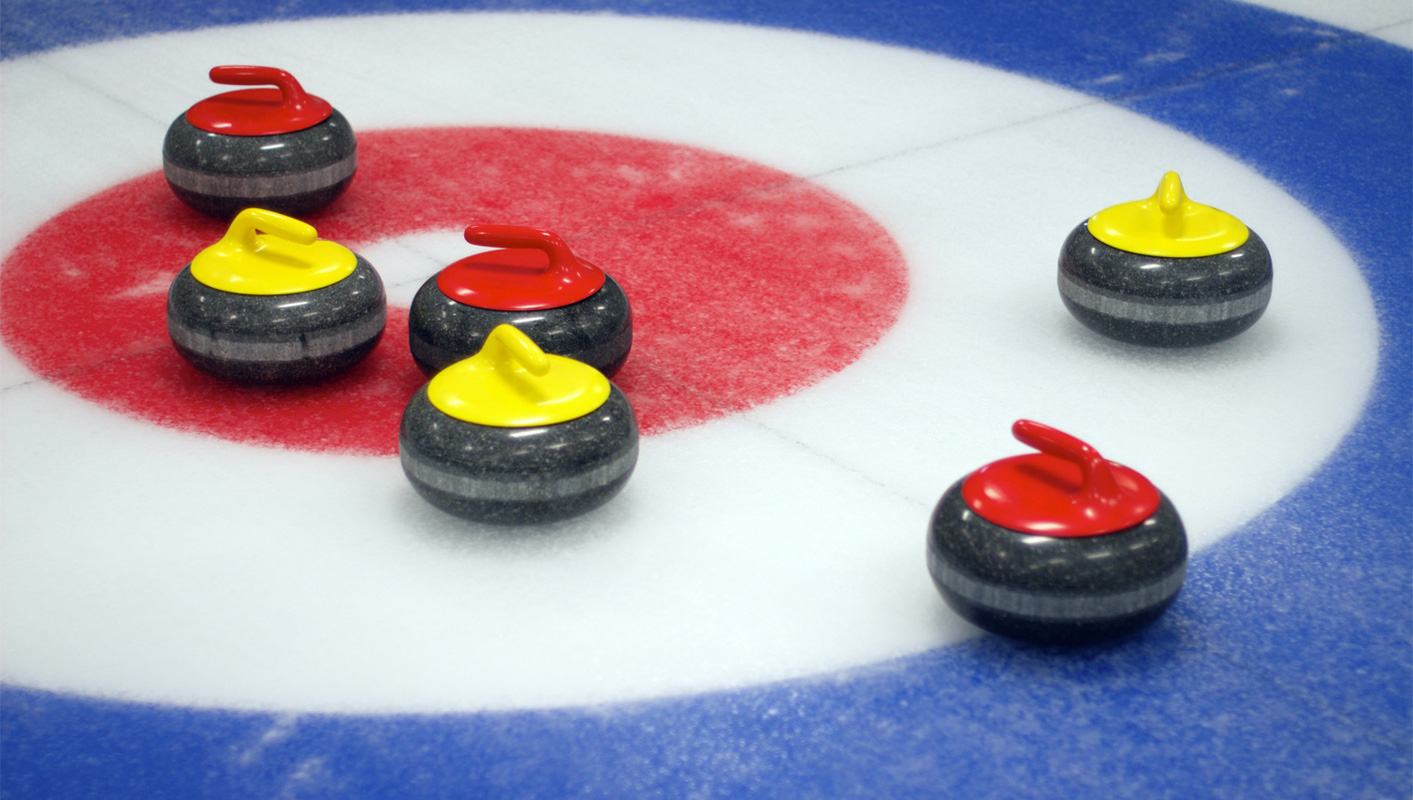
\includegraphics[width=\columnwidth]{img/curling2.jpg}
{\footnotesize Quando la pietra si ferma ha trasferito tutta la sua energia all'ambiente (aria e ghiaccio) come \alert{energia disordinata}:
\begin{itemize}
  \item i moti delle molecole d'aria avvengono in ogni direzione;
  \item tali moti avvengono con valori di velocità diversi;
  \item le forze intermolecolari hanno direzioni e intensità diverse.
\end{itemize}}}
\end{column}
\end{columns}
\end{frame}


\begin{frame}
  \frametitle{Dall'ordine al disordine}
L'esempio visto è assolutamente generalizzabile e ci permette di affermare che:
\begin{block}{Evoluzione di un sistema (1)}
  Nel corso del tempo, le forme ordinate di energia si trasformano spontaneamente in energia disordinata.
\end{block}
Perché?
\end{frame}

\section{Tempo}

\begin{frame}
  \frametitle{Verso del tempo (1)}
Immaginiamo di filmare una pallina che rimbalza contro le pareti di un recipiente. Potremmo mostrare il video così come è stato girato oppure al contrario e uno spettatore non saprebbe individuare il verso ``giusto'' del filmato.\\~\\{\pause}


Lo stesso vale per le particelle che compongono un gas, come affermato dalla teoria cinetica dei gas.
\end{frame}


\begin{frame}
  \frametitle{Verso del tempo (2)}
  
\begin{figure}
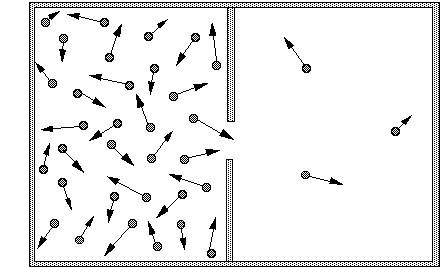
\includegraphics[width=.35\columnwidth]{img/scatolasetto.jpg}  
\end{figure}  
Immaginiamo un contenitore diviso a metà da un setto: una metà contiene del gas perfetto, l'altra no. Se togliamo il setto, il gas tenderà ad occupare tutto lo spazio disponibile.{\pause} Se un filmato di questo fenomeno venisse mostrato al contrario, sapremmo subito distinguerlo da quello ``corretto''.
\end{frame}

\begin{frame}
  \frametitle{Evoluzione}  
Concludiamo quindi che:
\begin{block}{Evoluzione di un sistema (2)}
Nonostante il modello per i gas abbia alla sua base la meccanica e pur essendo le leggi di quest'ultima simmetriche per inversione temporale, l'evoluzione del sistema nel tempo non è invertibile.
\end{block}\pause
Perché?

\end{frame}



\section{Stati}


\begin{frame}
\frametitle{Macrostati e microstati}
\begin{columns}
\begin{column}{0.3\textwidth}
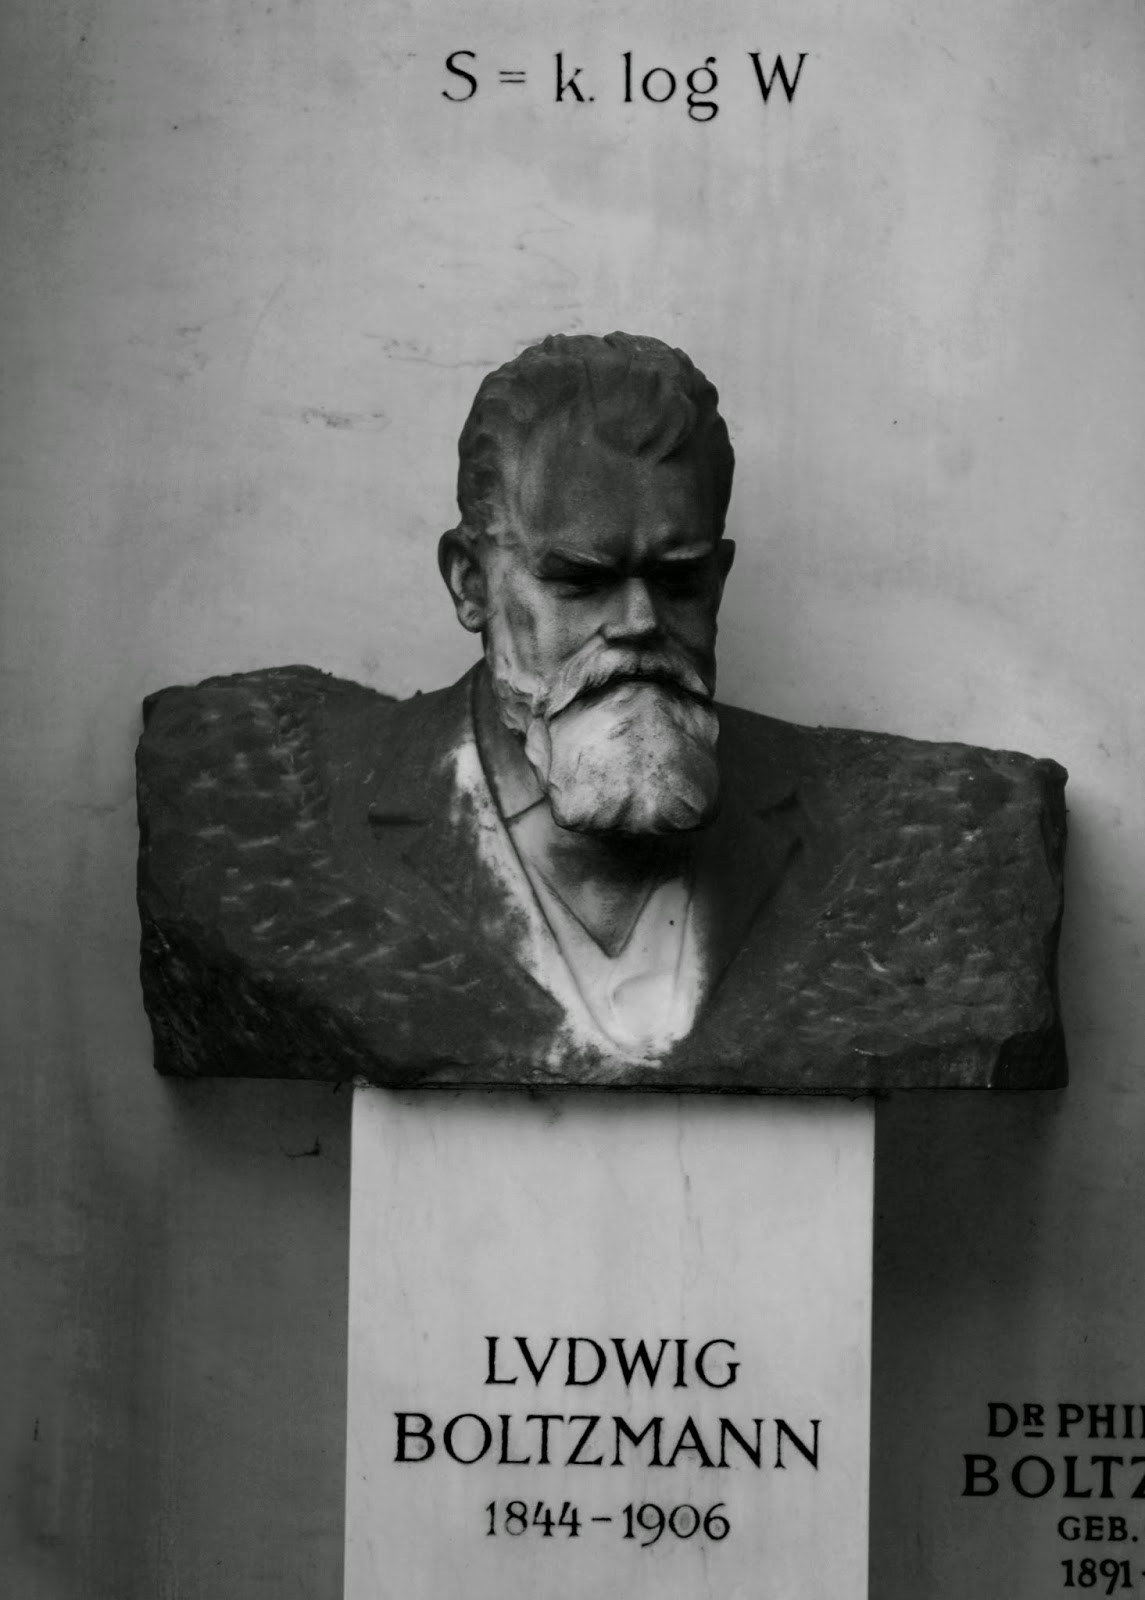
\includegraphics[width=\columnwidth]{img/boltzmann.jpg}
\end{column}
\begin{column}{0.7\textwidth}
Ludwig Boltzmann affronterà tale questione dal punto di vista statistico. Alla base del suo lavoro stanno i seguenti fatti:\pause
\begin{itemize}
\item<2-> ogni stato macroscopico è manifestazione di una configurazione microscopica (microstato);
\item<3-> ogni macrostato ha diversi microstati corrispondenti;
\item<4-> un macrostato è tanto più probabile quanti più microstati gli sono associati;
\item<5-> il numero di microstati è legato all'entropia di un certo macrostato del sistema.
\end{itemize}
\end{column}
\end{columns}
\end{frame}





\begin{frame}
\frametitle{Sistema modello}
Immaginiamo un sistema immensamente semplice, del quale possiamo valutare i diversi microstati.\pause\\~\\

Il sistema è composto da quattro particelle di gas perfetto (A, B, C e D), tutte uguali tra loro e quindi non distinguibili. Valutiamo la loro posizione, distinta tra ``sinistra'' e ``destra''.\pause\\~\\

Abbiamo cinque macrostati possibili.

\end{frame}




\begin{frame}
\frametitle{Macrostati possibili}

\begin{columns}
\begin{column}{0.5\textwidth}
\begin{figure}
\begin{tikzpicture}[scale=0.4]
\draw (0,0) -- (6,0) -- (6,3) -- (0,3) -- (0,0);
\draw (3,0) -- (3,3);

\draw [fill=purple, thick] (1,1) circle [radius=.2];

\draw [fill=purple, thick] (2,1) circle [radius=.2];

\draw [fill=purple, thick] (1,2) circle [radius=.2];

\draw [fill=purple, thick] (2,2) circle [radius=.2];
\end{tikzpicture}
$ A_{4,0} $
\end{figure}

\begin{figure}
\begin{tikzpicture}[scale=0.4]
\draw (0,0) -- (6,0) -- (6,3) -- (0,3) -- (0,0);
\draw (3,0) -- (3,3);

\draw [fill=purple, thick] (1,1) circle [radius=.2];

\draw [fill=purple, thick] (2,1) circle [radius=.2];

\draw [fill=purple, thick] (1,2) circle [radius=.2];

\draw [fill=purple, thick] (5,2) circle [radius=.2];
\end{tikzpicture}
$ A_{3,1} $
\end{figure}


\begin{figure}
\begin{tikzpicture}[scale=0.4]
\draw (0,0) -- (6,0) -- (6,3) -- (0,3) -- (0,0);
\draw (3,0) -- (3,3);

\draw [fill=purple, thick] (1,1) circle [radius=.2];

\draw [fill=purple, thick] (2,1) circle [radius=.2];

\draw [fill=purple, thick] (4,2) circle [radius=.2];

\draw [fill=purple, thick] (5,2) circle [radius=.2];
\end{tikzpicture}
$ A_{2,2} $
\end{figure}
\end{column}
\begin{column}{0.5\textwidth}





\begin{figure}
\begin{tikzpicture}[scale=0.4]
\draw (0,0) -- (6,0) -- (6,3) -- (0,3) -- (0,0);
\draw (3,0) -- (3,3);

\draw [fill=purple, thick] (1,1) circle [radius=.2];

\draw [fill=purple, thick] (5,1) circle [radius=.2];

\draw [fill=purple, thick] (4,2) circle [radius=.2];

\draw [fill=purple, thick] (5,2) circle [radius=.2];
\end{tikzpicture}
$ A_{1,3} $
\end{figure}


\begin{figure}
\begin{tikzpicture}[scale=0.4]
\draw (0,0) -- (6,0) -- (6,3) -- (0,3) -- (0,0);
\draw (3,0) -- (3,3);

\draw [fill=purple, thick] (4,1) circle [radius=.2];

\draw [fill=purple, thick] (5,1) circle [radius=.2];

\draw [fill=purple, thick] (4,2) circle [radius=.2];

\draw [fill=purple, thick] (5,2) circle [radius=.2];
\end{tikzpicture}
$ A_{0,4} $
\end{figure}

{\small Ogni macrostato può essere raggiunto mediante diversi microstati. Il numero di microstati associati ad $ A $ è indicato con $ W(A) $.}
\end{column}
\end{columns}
\end{frame}






\begin{frame}
\frametitle{Molteplicità dei macrostati (1)}

$ W = 1 $
\begin{tikzpicture}[scale=0.35]
\draw (0,0) -- (6,0) -- (6,3) -- (0,3) -- (0,0);
\draw (3,0) -- (3,3);

\draw [fill=purple, thick] (1,1) circle [radius=.2];
\node [below left] at (1,1) {{\tiny A}};

\draw [fill=purple, thick] (2,1) circle [radius=.2];
\node [below right] at (2,1) {{\tiny B}};

\draw [fill=purple, thick] (1,2) circle [radius=.2];
\node [above left] at (1,2) {{\tiny C}};

\draw [fill=purple, thick] (2,2) circle [radius=.2];
\node [above right] at (2,2) {{\tiny D}};
\end{tikzpicture}

~\\

$ W = 4 $
\begin{tikzpicture}[scale=0.35]
\draw (0,0) -- (6,0) -- (6,3) -- (0,3) -- (0,0);
\draw (3,0) -- (3,3);

\draw [fill=purple, thick] (1,1) circle [radius=.2];
\node [below left] at (1,1) {{\tiny A}};

\draw [fill=purple, thick] (2,1) circle [radius=.2];
\node [below right] at (2,1) {{\tiny B}};

\draw [fill=purple, thick] (1,2) circle [radius=.2];
\node [above left] at (1,2) {{\tiny C}};

\draw [fill=purple, thick] (5,2) circle [radius=.2];
\node [above right] at (5,2) {{\tiny D}};
\end{tikzpicture}
\begin{tikzpicture}[scale=0.35]
\draw (0,0) -- (6,0) -- (6,3) -- (0,3) -- (0,0);
\draw (3,0) -- (3,3);

\draw [fill=purple, thick] (1,1) circle [radius=.2];
\node [below left] at (1,1) {{\tiny A}};

\draw [fill=purple, thick] (2,1) circle [radius=.2];
\node [below right] at (2,1) {{\tiny B}};

\draw [fill=purple, thick] (1,2) circle [radius=.2];
\node [above left] at (1,2) {{\tiny D}};

\draw [fill=purple, thick] (5,2) circle [radius=.2];
\node [above right] at (5,2) {{\tiny C}};
\end{tikzpicture}
\begin{tikzpicture}[scale=0.35]
\draw (0,0) -- (6,0) -- (6,3) -- (0,3) -- (0,0);
\draw (3,0) -- (3,3);

\draw [fill=purple, thick] (1,1) circle [radius=.2];
\node [below left] at (1,1) {{\tiny A}};

\draw [fill=purple, thick] (2,1) circle [radius=.2];
\node [below right] at (2,1) {{\tiny D}};

\draw [fill=purple, thick] (1,2) circle [radius=.2];
\node [above left] at (1,2) {{\tiny C}};

\draw [fill=purple, thick] (5,2) circle [radius=.2];
\node [above right] at (5,2) {{\tiny B}};
\end{tikzpicture}
\begin{tikzpicture}[scale=0.35]
\draw (0,0) -- (6,0) -- (6,3) -- (0,3) -- (0,0);
\draw (3,0) -- (3,3);

\draw [fill=purple, thick] (1,1) circle [radius=.2];
\node [below left] at (1,1) {{\tiny D}};

\draw [fill=purple, thick] (2,1) circle [radius=.2];
\node [below right] at (2,1) {{\tiny B}};

\draw [fill=purple, thick] (1,2) circle [radius=.2];
\node [above left] at (1,2) {{\tiny C}};

\draw [fill=purple, thick] (5,2) circle [radius=.2];
\node [above right] at (5,2) {{\tiny A}};
\end{tikzpicture}

~\\

$ W = 6 $
\begin{tikzpicture}[scale=0.35]
\draw (0,0) -- (6,0) -- (6,3) -- (0,3) -- (0,0);
\draw (3,0) -- (3,3);

\draw [fill=purple, thick] (1,1) circle [radius=.2];
\node [below left] at (1,1) {{\tiny A}};

\draw [fill=purple, thick] (2,1) circle [radius=.2];
\node [below right] at (2,1) {{\tiny B}};

\draw [fill=purple, thick] (4,2) circle [radius=.2];
\node [above left] at (4,2) {{\tiny C}};

\draw [fill=purple, thick] (5,2) circle [radius=.2];
\node [above right] at (5,2) {{\tiny D}};
\end{tikzpicture}
\begin{tikzpicture}[scale=0.35]
\draw (0,0) -- (6,0) -- (6,3) -- (0,3) -- (0,0);
\draw (3,0) -- (3,3);

\draw [fill=purple, thick] (1,1) circle [radius=.2];
\node [below left] at (1,1) {{\tiny A}};

\draw [fill=purple, thick] (2,1) circle [radius=.2];
\node [below right] at (2,1) {{\tiny C}};

\draw [fill=purple, thick] (4,2) circle [radius=.2];
\node [above left] at (4,2) {{\tiny B}};

\draw [fill=purple, thick] (5,2) circle [radius=.2];
\node [above right] at (5,2) {{\tiny D}};
\end{tikzpicture}
\begin{tikzpicture}[scale=0.35]
\draw (0,0) -- (6,0) -- (6,3) -- (0,3) -- (0,0);
\draw (3,0) -- (3,3);

\draw [fill=purple, thick] (1,1) circle [radius=.2];
\node [below left] at (1,1) {{\tiny A}};

\draw [fill=purple, thick] (2,1) circle [radius=.2];
\node [below right] at (2,1) {{\tiny D}};

\draw [fill=purple, thick] (4,2) circle [radius=.2];
\node [above left] at (4,2) {{\tiny C}};

\draw [fill=purple, thick] (5,2) circle [radius=.2];
\node [above right] at (5,2) {{\tiny B}};
\end{tikzpicture}

~~~~~~~~~~\begin{tikzpicture}[scale=0.35]
\draw (0,0) -- (6,0) -- (6,3) -- (0,3) -- (0,0);
\draw (3,0) -- (3,3);

\draw [fill=purple, thick] (1,1) circle [radius=.2];
\node [below left] at (1,1) {{\tiny C}};

\draw [fill=purple, thick] (2,1) circle [radius=.2];
\node [below right] at (2,1) {{\tiny B}};

\draw [fill=purple, thick] (4,2) circle [radius=.2];
\node [above left] at (4,2) {{\tiny A}};

\draw [fill=purple, thick] (5,2) circle [radius=.2];
\node [above right] at (5,2) {{\tiny D}};
\end{tikzpicture}
\begin{tikzpicture}[scale=0.35]
\draw (0,0) -- (6,0) -- (6,3) -- (0,3) -- (0,0);
\draw (3,0) -- (3,3);

\draw [fill=purple, thick] (1,1) circle [radius=.2];
\node [below left] at (1,1) {{\tiny D}};

\draw [fill=purple, thick] (2,1) circle [radius=.2];
\node [below right] at (2,1) {{\tiny B}};

\draw [fill=purple, thick] (4,2) circle [radius=.2];
\node [above left] at (4,2) {{\tiny C}};

\draw [fill=purple, thick] (5,2) circle [radius=.2];
\node [above right] at (5,2) {{\tiny A}};
\end{tikzpicture}
\begin{tikzpicture}[scale=0.35]
\draw (0,0) -- (6,0) -- (6,3) -- (0,3) -- (0,0);
\draw (3,0) -- (3,3);

\draw [fill=purple, thick] (1,1) circle [radius=.2];
\node [below left] at (1,1) {{\tiny C}};

\draw [fill=purple, thick] (2,1) circle [radius=.2];
\node [below right] at (2,1) {{\tiny D}};

\draw [fill=purple, thick] (4,2) circle [radius=.2];
\node [above left] at (4,2) {{\tiny A}};

\draw [fill=purple, thick] (5,2) circle [radius=.2];
\node [above right] at (5,2) {{\tiny B}};
\end{tikzpicture}

\end{frame}







\begin{frame}
\frametitle{Molteplicità dei macrostati (2)}

$ W = 4 $
\begin{tikzpicture}[scale=0.35]
\draw (0,0) -- (6,0) -- (6,3) -- (0,3) -- (0,0);
\draw (3,0) -- (3,3);

\draw [fill=purple, thick] (1,1) circle [radius=.2];
\node [below left] at (1,1) {{\tiny A}};

\draw [fill=purple, thick] (5,1) circle [radius=.2];
\node [below right] at (5,1) {{\tiny B}};

\draw [fill=purple, thick] (4,2) circle [radius=.2];
\node [above left] at (4,2) {{\tiny C}};

\draw [fill=purple, thick] (5,2) circle [radius=.2];
\node [above right] at (5,2) {{\tiny D}};
\end{tikzpicture}
\begin{tikzpicture}[scale=0.35]
\draw (0,0) -- (6,0) -- (6,3) -- (0,3) -- (0,0);
\draw (3,0) -- (3,3);

\draw [fill=purple, thick] (1,1) circle [radius=.2];
\node [below left] at (1,1) {{\tiny B}};

\draw [fill=purple, thick] (5,1) circle [radius=.2];
\node [below right] at (5,1) {{\tiny A}};

\draw [fill=purple, thick] (4,2) circle [radius=.2];
\node [above left] at (4,2) {{\tiny C}};

\draw [fill=purple, thick] (5,2) circle [radius=.2];
\node [above right] at (5,2) {{\tiny D}};
\end{tikzpicture}
\begin{tikzpicture}[scale=0.35]
\draw (0,0) -- (6,0) -- (6,3) -- (0,3) -- (0,0);
\draw (3,0) -- (3,3);

\draw [fill=purple, thick] (1,1) circle [radius=.2];
\node [below left] at (1,1) {{\tiny C}};

\draw [fill=purple, thick] (5,1) circle [radius=.2];
\node [below right] at (5,1) {{\tiny B}};

\draw [fill=purple, thick] (4,2) circle [radius=.2];
\node [above left] at (4,2) {{\tiny A}};

\draw [fill=purple, thick] (5,2) circle [radius=.2];
\node [above right] at (5,2) {{\tiny D}};
\end{tikzpicture}
\begin{tikzpicture}[scale=0.35]
\draw (0,0) -- (6,0) -- (6,3) -- (0,3) -- (0,0);
\draw (3,0) -- (3,3);

\draw [fill=purple, thick] (1,1) circle [radius=.2];
\node [below left] at (1,1) {{\tiny D}};

\draw [fill=purple, thick] (5,1) circle [radius=.2];
\node [below right] at (5,1) {{\tiny B}};

\draw [fill=purple, thick] (4,2) circle [radius=.2];
\node [above left] at (4,2) {{\tiny C}};

\draw [fill=purple, thick] (5,2) circle [radius=.2];
\node [above right] at (5,2) {{\tiny A}};
\end{tikzpicture}

~\\

$ W = 1 $
\begin{tikzpicture}[scale=0.35]
\draw (0,0) -- (6,0) -- (6,3) -- (0,3) -- (0,0);
\draw (3,0) -- (3,3);

\draw [fill=purple, thick] (4,1) circle [radius=.2];
\node [below left] at (4,1) {{\tiny A}};

\draw [fill=purple, thick] (5,1) circle [radius=.2];
\node [below right] at (5,1) {{\tiny B}};

\draw [fill=purple, thick] (4,2) circle [radius=.2];
\node [above left] at (4,2) {{\tiny C}};

\draw [fill=purple, thick] (5,2) circle [radius=.2];
\node [above right] at (5,2) {{\tiny D}};
\end{tikzpicture}
\end{frame}


\begin{frame}
  \frametitle{Frequenza dei macrostati}
  Riassumiamo in un grafico la frequenza dei macrostati:
  \begin{figure}
    \begin{tikzpicture}[scale=0.5]
    
\draw (0,7) -- (0,0) -- (12,0);
\draw [fill=purple] (1,0) rectangle (3,1);
\node [below] at (2,0) {{\tiny $ A_{4,0} $}};
\draw [fill=purple] (3,0) rectangle (5,4);
\node [below] at (4,0) {{\tiny $ A_{3,1} $}};
\draw [fill=purple] (5,0) rectangle (7,6);
\node [below] at (6,0) {{\tiny $ A_{2,2} $}};
\draw [fill=purple] (7,0) rectangle (9,4);
\node [below] at (8,0) {{\tiny $ A_{1,3} $}};
\draw [fill=purple] (9,0) rectangle (11,1);
\node [below] at (10,0) {{\tiny $ A_{0,4} $}};
\draw [dotted] (0,1) -- (1,1);
\node [left] at (0,1) {{\tiny $ W=1 $}};
\draw [dotted] (0,4) -- (3,4);
\node [left] at (0,4) {{\tiny $ W=4 $}};
\draw [dotted] (0,6) -- (5,6);
\node [left] at (0,6) {{\tiny $ W=6 $}};
\end{tikzpicture}
  \end{figure}
\end{frame}

\begin{frame}
  \frametitle{Probabilità dei macrostati (1)}
   Nel caso considerato ci sono $ 2^4 = 16 $ microstati possibili, $ 6 $ dei quali associati al macrostato $ A_{2,2} $.\pause Tale stato ha una probabilità di verificarsi del:
   \begin{center}
   $ \frac{1}{16} \cdot 6 = \frac{6}{16} = 0,375 = 37,5 \% $ 
   \end{center}
   di verificarsi, ed è quindi lo stato più probabile.\pause\\
   Gli stati $ A_{4,0} $ e $ A_{0,4} $ hanno probabilità del 
   \begin{center}
   $ \frac{1}{16} \cdot 1 = \frac{1}{16} = 0,0625 = 6,25 \% $ 
   \end{center}
  e sono quindi i meno probabili.
\end{frame}


\begin{frame}
  \frametitle{Probabilità dei macrostati (2)}
Se nel nostro sistema ci fossero $ 8 $ particelle avremmo $ 2^8 = 256 $ microstati possibili.{\pause} Il macrostato $ A_{4,4} $ avrebbe $ 70 $ microstati associati e avrebbe quindi una possibilità di verificarsi del:
      \begin{center}
   $ \frac{1}{256} \cdot 70 = \frac{70}{256} = 0,273 = 27,3 \% $ 
   \end{center}{\pause}
Gli stati meno probabili saranno ovviamente $ A_{8,0} $ e $ A_{0,8} $, con una probabilità dello:
      \begin{center}
   $ \frac{1}{256} \cdot 1 = \frac{1}{256} = 0,0039 = 0,39 \% $ 
   \end{center}\pause
   Immaginiamo la situazione nel caso di $ N_A $ molecole!
\end{frame}



\begin{frame}
  \frametitle{Evoluzione del sistema}
  Il sistema evolve quindi \alert<1>{da stati meno probabili a stati più probabili}. In questo caso, vediamo le molecole disperdersi uniformemente nello spazio.\\\pause~\\Il caso contrario, in cui tutte le particelle si trovano da una stessa parte, \alert<2>{non è impossibile}, è solo \alert<2>{altamente improbabile}.
\end{frame}

\begin{frame}
\frametitle{Disordine}
  Interpretiamo allora con questa idea il concetto di \alert<1-2>{disordine}:
  \begin{itemize}
    \item lo stato $ A_{8,0} $ è più ordinato perché abbiamo la minima indeterminazione sulla posizione delle particelle (lo stesso vale per $ A_{0,8} $);\pause
    \item lo stato $ A_{4,4} $ è più disordinato perché abbiamo la massima indeterminazione sulla posizione delle particelle.\pause
  \end{itemize}
  \begin{block}{Concludiamo che:}
    più un microstato è disordinato, maggiore è la probabilità che esso si verifichi spontaneamente.
  \end{block}
\end{frame}

\section{Boltzmann}

\begin{frame}
  \frametitle{Equazione di Boltzmann}
  Ludwig Boltzmann dimostra nel 1877 che l'entropia $ S(A) $ del macrostato $ A $ è data da:
  \begin{center}
\colorbox{blue!30}{$ S(A) = k_B \ln W(A) $}
\end{center}
con:
\begin{itemize}
  \item $ k_B = \text{costante di Boltzmann} = 1,38 \times 10^{-23} \, \frac{J}{K}  $;
  \item il valore di riferimento $ 0 \, \frac{J}{K} $ assegnato ad un cristallo perfetto di atomi uguali tra loro alla temperatura di $ 0 \, K $.
\end{itemize}
\end{frame}

\begin{frame}
\frametitle{Ancora il secondo principio}
  Possiamo trovare allora la spiegazione dell'enunciato dell'entropia del secondo principio nel fatto che la funzione precedente è crescente (nel tempo) e pertanto che:
\begin{block}{Conclusione}
  L'entropia di un sistema tende ad aumentare man mano che il sistema si evolve spontaneamente verso macrostati più probabili.
\end{block}
\end{frame}


\section{Principi}

\begin{frame}
  \frametitle{Principi della termodinamica (1)}
  \begin{block}{Principio zero}
    Se il corpo A è in equilibrio termico con un corpo C e anche un altro corpo B è in equilibrio termico con C, allora A e B risultano in equilibrio termico tra loro.
  \end{block}
\end{frame}

\begin{frame}
  \frametitle{Principi della termodinamica (2)}
  \begin{block}{Primo principio}
    L'energia totale di un sistema si conserva: 
    \begin{center}
\colorbox{blue!30}{$ \Delta U = Q - L $}
\end{center}
  \end{block}
\end{frame}


\begin{frame}
  \frametitle{Principi della termodinamica (3)}
  \begin{block}{Secondo principio}
    \textbf{Kelvin:} È impossibile realizzare una trasformazione il cui \emph{unico} risultato sia quello di assorbire una determinata quantità di calore da un’\emph{unica} sorgente e trasformarla \emph{integralmente} in lavoro.\\
    \textbf{Clausius:} È impossibile realizzare una trasformazione il cui \emph{unico} risultato sia quello di fare passare calore da un corpo più freddo a uno più caldo.\\
    \textbf{Rendimento:} È impossibile progettare una macchina termica che abbia rendimento uguale a 1.\\
    \textbf{Entropia:} L'evoluzione spontanea di un sistema isolato giunge a uno stato di equilibrio a cui corrisponde il massimo aumento dell’entropia (compatibile con il rispetto del primo principio della termodinamica).
  \end{block}
\end{frame}


\begin{frame}
  \frametitle{Principi della termodinamica (4)}
  La temperatura più bassa mai raggiunta dall'uomo è stata di $ 0,45 \, nK $ (meno di un miliardesimo di Kelvin, raggiunta nel 2003 al MIT).\pause\\~\\
  
Gli esperimenti mostrano che più ci si avvicina allo zero assoluto, più risulta difficile raffreddare ulteriormente un corpo, fino a diventare praticamente impossibile.{\pause} Il terzo principio riassume questo fatto:
  \begin{block}{Terzo principio (1907)}
    È impossibile raffreddare un corpo fino allo zero assoluto mediante una procedura che contiene un numero finito di trasformazioni.
  \end{block}
\end{frame}





\end{document}
